\documentclass[12pt]{report}

\usepackage{graphicx}
\usepackage[spanish,mexico]{babel}
\usepackage[utf8]{inputenc}
\usepackage{amsmath}
\usepackage{fancyhdr}
\usepackage{float}
\usepackage{jslisting}
\usepackage{jslistings}

\usepackage[acronym, toc]{glossaries}
\usepackage{biblatex}
\addbibresource{references.bib}

\graphicspath{ {./images/} }

\renewcommand{\glstextformat}[1]{\textit{#1}}
\makeglossaries
\newglossaryentry{frontend}
{
    name=frontend,
    description={Se encarga de la parte del software que interactúa con el usuario y que el usuario puede ver.}
}
\newglossaryentry{backend}
{
    name=backend,
    description={Representa la capa de acceso de datos.}
}

\newacronym{ajax}{AJAX}{Asynchronous JavaScript And XML (JavaScript asíncrono y XML)}
\newacronym{spa}{SPA}{Single Page Application (Aplicación de una sola página)}
\newacronym{epel}{EPEL}{Extra Packages for Enterprise Linux (Paquetes Extra para Linux Empresarial)}
\newacronym{jit}{JIT}{Just In Time (Justo A Tiempo)}
\newacronym{npm}{NPM}{Node Package Manager (Administrados de Paquetes Node)}
\newacronym{dom}{DOM}{Document Object Model (Modelo de Objeto de Documento)}
\newacronym{rdbms}{RDBMS}{Relational Database Management System (Sistema de Gestión de Bases de Datos Relacionales)}
\newacronym{rest}{REST}{Representational State Transfer (Transferencia de Estado Representacional)}
\newacronym{api}{API}{Application Programming Interface (Interfaz de Programación de Aplicaciones)}
\newacronym{crud}{CRUD}{Create, Read, Update, and Delete (Crear, Leer, Actualizar y Borrar)}

\newglossaryentry{mixin}
{
    name=mixin,
    plural=mixins,
    description={En los lenguajes de programación orientada a objetos, un mixin es una clase que ofrece cierta funcionalidad para ser heredada por una subclase, pero no está ideada para ser autónoma.}
}

\newglossaryentry{ionic}
{
    name=ionic,
    description={SDK completo de código abierto para el desarrollo de aplicaciones móviles híbridas}
}
\newglossaryentry{token}
{
    name=token,
    description={Un objeto del sistema que representa el sujeto de las operaciones de control de acceso}
}
\newglossaryentry{websocket}
{
    name=websocket,
    plural=websockets,
    description={Protocolo de comunicaciones informáticas que proporciona canales de comunicación dúplex completo a través de una única conexión TCP}
}
\newglossaryentry{axios}
{
    name=axios,
    description={Cliente HTTP basado en promesas para el navegador y Node.js}
}
\newglossaryentry{cookie}
{
    name=cookie,
    plural=cookies,
    description={Es una pequeña pieza de datos enviada desde un sitio web y almacenada en la computadora del usuario por el navegador web del usuario mientras el usuario está navegando}
}
\newglossaryentry{daemon}
{
    name=daemon,
    description={En los sistemas operativos de computadora multitarea, un daemon es un programa informático que se ejecuta como un proceso en segundo plano}
}
\newglossaryentry{escalabilidad}
{
    name=escalabilidad,
    description={Es un anglicismo que describe la capacidad de un negocio o sistema de crecer en magnitud}
}
\newglossaryentry{framework}
{
    name=framework,
    plural=frameworks,
    description={Un framework, entorno de trabajo​ o marco de trabajo​ es un conjunto estandarizado de conceptos, prácticas y criterios para enfocar un tipo de problemática particular que sirve como referencia, para enfrentar y resolver nuevos problemas de índole similar}
}
\newglossaryentry{hardware}
{
    name=hardware,
    description={Se refiere a las partes físicas, tangibles, de un sistema informático}
}
\newglossaryentry{software}
{
    name=software,
    description={Soporte lógico de un sistema informático, que comprende el conjunto de los componentes lógicos necesarios que hacen posible la realización de tareas específicas}
}
\newglossaryentry{holístico}
{
    name=holístico,
    description={Del todo o que considera algo como un todo}
}
\newglossaryentry{hook}
{
    name=hook,
    plural=hooks,
    description={Datos y comandos ejecutables enviados de una aplicación a otra a través de HTTP}
}
\newglossaryentry{isomorfico}
{
    name=isomórfico,
    plural=isomórficos,
    description={El isomorfismo aplicado al desarrollo web significa renderizar páginas tanto en el lado del servidor como del cliente}
}
\newglossaryentry{kernel}
{
    name=kernel,
    description={Programa de computadora que es el núcleo del sistema operativo de una computadora, con control completo sobre todo en el sistema}
}
\newglossaryentry{minificacion}
{
    name=minificación,
    description={el proceso mediante el cual se eliminan datos innecesarios o redundantes de un recurso sin que se vea afectada la forma en que los navegadores lo procesan}
}
\newglossaryentry{plugin}
{
    name=plugin,
    plural=plugins,
    description={Es un componente de software que agrega una característica específica a un programa de computadora existente}
}
\newglossaryentry{renderizado}
{
    name=renderizado,
    description={Proceso de renderizar}
}
\newglossaryentry{renderizar}
{
    name=renderizar,
    description={Proceso de generar un modelo visual a partir de una información dada}
}
\newglossaryentry{script}
{
    name=script,
    description={Lista de comandos que ejecuta un determinado programa o motor de secuencias de comandos}
}
\newglossaryentry{singleton}
{
    name=singleton,
    description={Patrón de diseño de software que restringe la creación de instancias de una clase a una instancia única}
}
\newglossaryentry{tablet}
{
    name=tablet,
    description={Computadora portátil de mayor tamaño que un teléfono inteligente o un PDA, se trata de una sola pieza que integra una pantalla táctil (sencilla o multitáctil) que emite luz y con la que se interactúa primariamente con los dedos}
}

\setlength{\oddsidemargin}{0in}
\setlength{\textwidth}{6in}
\setlength{\topmargin}{0in}
% \setlength{\voffset}{0.5in}
\setlength{\voffset}{0in}
\setlength{\headheight}{0.25in}
\setlength{\headsep}{0.5in}
\setlength{\hoffset}{0.5in}
% \setlength{\textheight}{8in}
\setlength{\textwidth}{5.5in}
\setlength{\topskip}{0in}
\setlength{\footskip}{1in}
\setlength{\parskip}{2ex}

\definecolor{codegray}{gray}{0.5}
\definecolor{codebox}{gray}{0.95}
\newcommand{\code}[1]{\colorbox{codebox}{\textcolor{codegray}{\texttt{#1}}}}

\title{
   {“Diseño y desarrollo de sistema multi-plataforma para gestión de ventas y logística de microempresa.”}\\
   {\large INSTITUTO TECNOLÓGICO DE TIJUANA}\\
   {
\includegraphics{escudo1.png}}
}
\author{José Luis Murillo Ríos}
\date{21 DE JUNIO DEL 2019}

% \fancyhead{}
% \fancyfoot{}
% \renewcommand{\headrulewidth}{0pt}
% \fancyhead[RO,LE]{\footnotesize\thepage}
% \fancyhead[RE]{\footnotesize\slshape\leftmark}

% \fancyhead{\fontsize{8}{10}\selectfont\nouppercase\rightmark}
\newcommand{\changefont}{\fontsize{10}{12}\selectfont}

\fancyhf{}

\fancyhead[L]{\changefont \slshape \nouppercase\leftmark}
\fancyfoot[R]{\changefont \slshape \thepage}
% \fancyfoot[L]{\changefont \slshape \nouppercase\rightmark}

\renewcommand{\headrulewidth}{0.5pt}
\renewcommand{\footrulewidth}{0.5pt}

\pagestyle{fancy}

% \rhead{\leftmark}
% \cfoot{\thepage}

\begin{document}
\setcounter{page}{1}
\pagenumbering{roman}
\thispagestyle{empty}
\begin{center}
   INSTITUTO TECNOLÓGICO DE TIJUANA\\[0.75cm]
   Ingeniería en Sistemas Computacionales\\[0.8in]
\end{center}
\begin{figure}[h]
\begin{center}


\includegraphics[height=5.5 cm]{escudo1.png}
\vspace{0cm}
\end{center}
\end{figure}
\vspace{1cm}
\begin{center}
DISEÑO Y DESARROLLO DE SISTEMA MULTI-PLATAFORMA PARA GESTIÓN DE VENTAS Y LOGÍSTICA DE MICROEMPRESA.\\[4mm]
POR\\[4mm]
JOSÉ LUIS MURILLO RÍOS\\[1cm]
\small PARA OBTENER EL TÍTULO DE INGENIERO EN SISTEMAS COMPUTACIONALES
\vfill
TIJUANA, B.C. \hfill AGOSTO 2019
\end{center}

\newpage
\thispagestyle{empty}
\begin{center}
DISEÑO Y DESARROLLO DE SISTEMA MULTI-PLATAFORMA PARA GESTIÓN DE VENTAS Y LOGÍSTICA DE MICROEMPRESA.\\[1.3cm]
POR\\[0.8cm]
JOSÉ LUIS MURILLO RÍOS\\[0.8cm]
\small AGOSTO 2019\\[0.7cm]
\end{center}

% \chapter*{RESUMEN}
\newpage

\begin{center}
  {\Large \bf{RESUMEN}}
\end{center}
Cada día mas emprendedores inician su negocio con la ayuda de servcicios de venta en linea; muchas de estas empresas 
tienden a crecer y requerir de sistemas mas especializados que se ajusten a necesidades particulares.\\[0.8cm]
Se desarrolla un sistema que tiene como objetivo el llevar control de los procesos de venta y logística de una empresa.
El propósito del proyecto es integrar los servicios existentes de venta en linea de la compañía
y extender su uso, adaptándalos a los requerimientos específicas del cliente, así como diseñar una interfáz gráfica que permita
proporcionar un servicio mas rápido y agilice los proceso de elaboracion y entrega de productos.
 
% \chapter*{DEDICATORIA}
\newpage
\begin{center}
  {\Large  \bf{DEDICATORIA}}
\end{center}
\begin{center}
  A mis abuelos, por creer siempre en mi\\
  Gracias
\end{center}

 
% \chapter*{AGRADECIMIENTOS}
\newpage
\begin{center}
  {\Large  \bf{AGRADECIMIENTOS}}
\end{center}
\begin{center}
  Quiero dar gracias a Bolt Media por incluirme en su equipo y darme la oportunidad de crecer.
\end{center}


\newpage
\tableofcontents

\newpage
\listoftables
\addcontentsline{toc}{chapter}{Índice de Tablas} %%% Para introducir una línea en el índice
\listoffigures
\addcontentsline{toc}{chapter}{Índice de Figuras}
\lstlistoflistings

\chapter{Introducción}
\pagenumbering{arabic} %%% esto es para regresar el modo de numeración a numeración arábiga
\setcounter{page}{1}  %%% empezamos en página 1
\thispagestyle{empty}  %%%% la primera página no va enumerada

Muchas pequeñas empresas dependen en gran medida al éxito de sus ventas en linea, por lo que adoptan el uso de tecnologías robustas (como Shopify y WooCommerce) para su administración. su función principal es servir como puntos de entrada para los clientes pero dichos servicios no están diseñados para mostrar información detallada a distintas áreas de la empresa. Cada día mas emprendedores inician su negocio con la ayuda de estos servicios de venta en linea; algunos de estos negocios tienden a crecer y requerir de sistemas mas especializados que se ajusten a necesidades particulares.

\section{Antecedentes y definición del problema}
Se solicitó a la empresa Bolt Media Internacional S. de R.L. de C.V. desarrollar una plataforma que conectara las transacciones de rosesland.com, una plataforma de ventas en linea desarrollada en Shopify a las operaciones internas de la florería, como lo son las ventas de mostrador, la manufactura y la entrega de los productos.
\vspace{0.8cm}
Actualmente la florería realiza todo este proceso con comandas que los empleados de ventas llenan a mano, para después enviarlos al área de elaboración de arreglos florales y posteriormente se entregan al encargado de logística para dar indicaciones de la distribución de los productos. Este proceso de venta es lento y genera una experiencia poco placentera para los compradores, a su vez el área de manufactura está conformado por artesanos y trabajadores del campo que tienen un nivel de comprensión de lectura bajo y pueden llegar a cometer errores que retrasen todos los procesos. Por tales motivos este sistema debe ser fácil de usar para usuarios de distintas áreas y a su vez el diseño debe de adaptarse tanto a diferentes tamaños de pantallas como a diferentes dispositivos móviles. Se requiere una base de datos que notifique en tiempo real los cambios
en la información asi como un servidor que administre los permisos adecuados para su manipulación.

\section{Motivación para atender el problema}
Una de las herramientas mas poderosas para el comercio es el internet, 
saber aprovecharlo genera importantes beneficios para cualquier negocio, 
es por ello que la empresa Rosesland debe adoptar un proceso mas automatizado
en sus funciones y tomar ventaja de los ordenadores y dispositivos con los que cuenta la empresa.

\section{Propuesta de solución}
Implementar un sistema diseñado principalmente para ser utilizado en pantallas táctiles
que muestre las transacciones realizadas durante el día tanto en mostrador como en la pagina web,
dando un informe detallado de las operaciones de la compañia.

\section{Objetivos generales}
Automatizar el proceso de ventas y entregas de la floreía Rosesland 
e integrar los servicios de su tienda en linea rosesland.com 
mediante una aplicación web progresiva, que sea compatible con los dispositivos existentes de la empresa
y que funcione adecuadamente en navegadores de internet modernos.

\section{Objetivos específicos}
\begin{enumerate}
\item Desarrollar un servidor que adminstre la autenticación de los empleados y su acceso a la información.
\item Implementar una base de datos que notifique a los usuarios cambios en la información en tiempo real.
\item Diseñar una aplicacion web progesiva que garantice una experiencia de usuario óptima para todas las areas de la empresa
\item Integrar los servicios de la tienda en linea rosesland.com con las operaciones internas de la empresa, uniendo los procesos en una sola plataforma
\end{enumerate}


\chapter{Marco teórico}
\thispagestyle{fancy}
\pagenumbering{arabic} %%% esto es para regresar el modo de numeración a numeración arábiga
\setcounter{page}{1}  %%% empezamos en página 1
\thispagestyle{empty}  %%%% la primera página no va enumerada
Un \textbf{\textit{stack de aplicaciones}} es una colección de software o tecnologías que se utilizan para crear una aplicación web. Las aplicaciones de una sola página (SPA - Single Page Application) han crecido en popularidad ya que proporcionan una experiencia de usuario más fluida: llamadas de servidor livianas cambian lo que se muestra en la pantalla sin tener que actualizar toda la página. El resultado parece bastante ingenioso en comparación con la antigua forma de volver a cargar la página por completo. Esto provocó un aumento en los \textit{frameworks} de \textit{front-end}, ya que gran parte del trabajo se realizó en el lado del cliente. Aproximadamente al mismo tiempo, aunque completamente sin relación, las bases de datos NoSQL también comenzaron a ganar popularidad. El término \textit{stack} fue popularizado por primera vez por LAMP Stack: Linux, Apache, MySQL y PHP. Linux es el sistema operativo, Apache actúa como el servidor HTTP, MySQL proporciona la base de datos relacional para manejar la información de la aplicación y PHP es el lenguaje de programación en el que se construye la aplicación. MERN es un paquete de software que significa MongoDB, ExpressJS, ReactJS y NodeJS. Juntos, estos programas gratuitos mejoran la simplicidad del proceso de desarrollo web. Las opciones son muchas, pero elegir una puede ser difícil.

\chapter{Análisis y diseño del sistema}
Las microempresas constituyen una potencia impulsora y se consideran entre las principales fuentes de trabajo, no obstante, es muy común encontrar microempresas con dificultades de crecimiento, principalmente debido a una mala administración o por falta de aprovechamiento de sus recursos. \\[0.8cm]
A continuación se describen los procedimientos necesarios para elaborar un sistema que permita a la empresa Rosesland llevar control de las ventas, elaboración y entrega de productos, así como incorporar los servicios de su tienda en linea al sistema. Permitiendo a la empresa tomar ventaja de las tecnologías web mas recientes, aprovechando al máximo los recursos existentes de la compañia.

\section{E-Commerce (Comercio electrónico)}
El comercio electrónico se refiere al proceso de compra o venta de productos o servicios a través de Internet. Las compras en línea se están volviendo cada vez más populares debido a la velocidad y facilidad de uso para los clientes. Las actividades de comercio electrónico, como la venta en línea, pueden dirigirse a consumidores u otras empresas. Vender en línea puede ayudar a su empresa a llegar a nuevos mercados y aumentar sus ventas e ingresos (ya sea a través de su propio sitio web o de un sitio de mercado electrónico).

\begin{figure}[H]
  \centering
  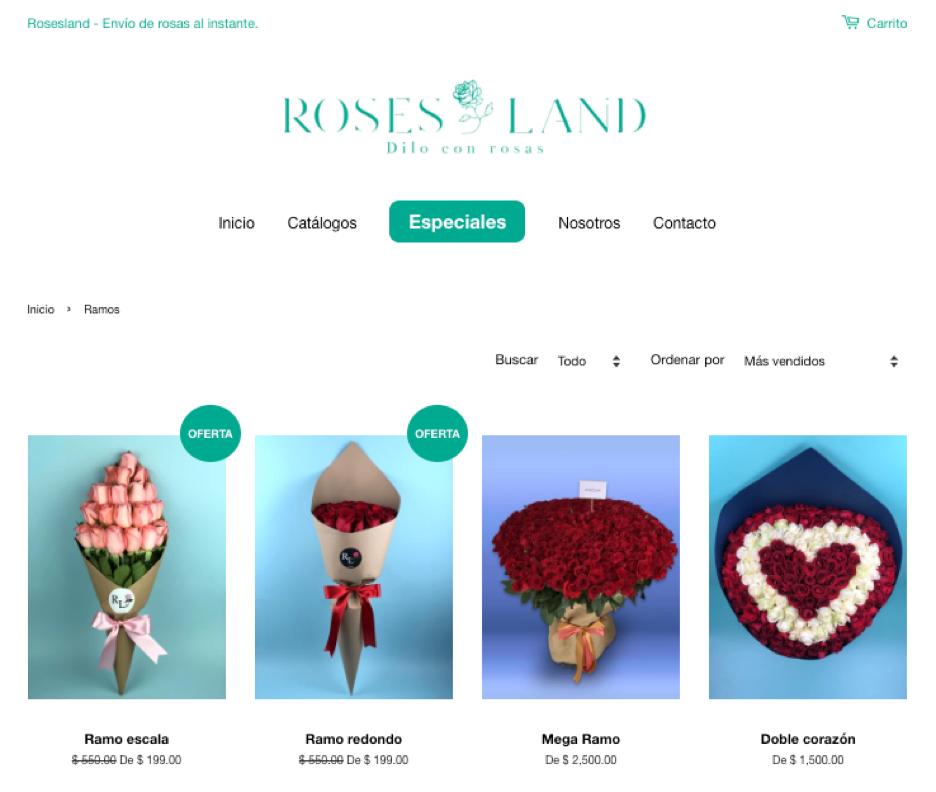
\includegraphics[width=0.9\textwidth]{rosesland}
  \caption{Tienda en linea actual de la empresa.}
\end{figure}

\subsubsection{Shopify}
Shopify es un servicio web que le permite configurar una tienda en línea para vender sus productos. 
Le da la facilidad organizar sus productos, personalizar el diseño de su tienda, 
aceptar pagos con tarjeta de crédito, rastrear y responder a pedidos. 
Shopify.com permite a los vendedores elegir entre opciones de diseño gratuitas 
o diseños personalizados creados por los usuarios.

\begin{figure}[H]
  \centering
  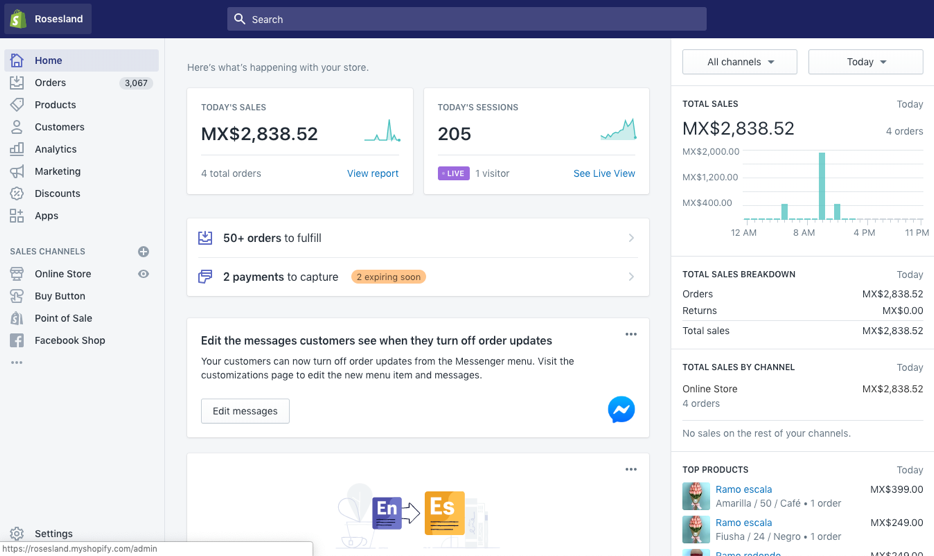
\includegraphics[width=0.9\textwidth]{shopify}
  \caption{Interfaz del administrador Shopify.}
\end{figure}

\section{Requerimientos del proyecto}
El producto final está enfocado en incrementar las ventas de la empresa Rosesland, con la ayuda de una plataforma que administre y mejore sus procesos internos. La finalidad del proyecto es disminuir los tiempos de ventas, elaboración y entrega de productos, así como la de crear un vínculo entre el servidor y su infraestructura actual extendiendo sus capacidades.
\vspace{0.8cm}

El sistema debe adaptarse al sistema operativo Linux. Anticipado a futuros cambios en la plataforma se decide trabajar con Node.js, ya que es de código abierto y multiplataforma, esto permite beneficiarse de la reutilización del código y la falta de cambio de contexto. Las aplicaciones Node.js están escritas en JavaScript puro y pueden ejecutarse dentro del entorno Node.js en Windows, Linux, etc.
\vspace{0.8cm}

La interfaz gráfica de usuario de la aplicación debe ser responsiva y funcionar en la mayoría de los navegadores web modernos, además debe ser fácil de aprender, idealmente requerir poco entrenamiento.
\vspace{0.8cm}

\subsection{Herramientas}
Node.js permite incorporar herramientas poderosas a proyectos de cualquier tipo. Esto incluye todo, desde bibliotecas y \glspl{framework} como jQuery y AngularJS hasta procesadores de código como Webpack. Los paquetes vendrán en una carpeta típicamente llamada node\_modules, que también contendrá un archivo package.json. Este archivo contiene información sobre todos los paquetes, incluidas las dependencias, que son módulos adicionales necesarios para usar un paquete en particular.

\subsubsection{Dependencias de desarrollo}
Las dependencias de desarrollo son aquellas que se utilizan dentro del entorno de programación. Aquí se incluyen herramientas que no forman parte del ejecutable final como lo son lo preprocesadores, empaquetadores y analistas de código. Los principales módulos de desarrollo son los siguientes:
\begin{itemize}
  \item Babel: es un compilador de JavaScript utilizado para convertir código ECMAScript 2015+ (ES6+) en una versión que pueda ser ejecutado en motores JavaScript más antiguos.
  \item Webpack: es un empaquetador de módulos principalmente para JavaScript, pero puede transformar archivos \gls{frontend} como HTML, CSS e imágenes si se incluyen los complementos correspondientes.
  \item ESLint: es una herramienta de análisis de código estático para identificar patrones problemáticos encontrados en el código JavaScript.
  \item PostCSS: es una herramienta de desarrollo de software que utiliza complementos basados en JavaScript para automatizar las operaciones de rutina de CSS. Con este modulo es posible analizar CSS, agregar prefijos de proveedor a las reglas CSS, ejecutar optimizaciones enfocadas, para garantizar que el resultado final sea lo más pequeño posible para un entorno de producción.
  \item Pug: es un preprocesador que simplifica la tarea de escribir HTML. También agrega funcionalidades, como objetos Javascript, condiciones, bucles, \glspl{mixin} y plantillas.
\end{itemize}

\subsubsection{Estructura del proyecto}
La estructura del proyecto Node.js está influenciada por preferencias personales, la arquitectura del proyecto y la estrategia de inyección de módulos que se está utilizando. Para tener una estructura FERN, es imperativo separar el código fuente del servidor y el utilizado por el cliente, ya que el código del lado del cliente o \gls{frontend} probablemente se minimizará y se enviará al navegador y es público en su naturaleza básica. Y el lado del servidor o el \gls{backend} proporcionarán \acrshort{api} para realizar operaciones \acrshort{crud}.

\subsubsection{Directorios}
\begin{itemize}
  \item node\_modules: Directorio oculto que contiene las dependencias generales del proyecto, este archivo debe ser ignorado por el controlador de versiones.
  \item server: Aquí se encuentran los archivos requeridos por el servidor para el enrutamiento, la conexión con la base de datos y las funciones de utilidad del \gls{backend}.
  \item src: Este directorio concentra todos los elementos necesarios para producir nuestra aplicación cliente.
  \item views: En esta carpeta se incluyen los templates necesarios para generar las vistas HTML de nuestro proyecto.
  \item www: Su propósito es contener los archivos del cliente, aquí podemos encontrar el código de producción de nuestra aplicación web compilado y minificado, así como las hojas de estilo, imágenes, fuentes tipográficas, vectores, etc.
\end{itemize}

\subsubsection{Archivos principales}
\begin{itemize}
  \item .babelrc: Contiene los mecanismos necesarios para compilar sintaxis moderna de JavaScript y una lista con los navegadores web a los que se requiere dar enfoque.
  \item .env: Documento oculto que contiene las variables del entorno, este archivo es ignorado por el controlador de versiones.
  \item .eslintrc.js: En este archivo se declaran las reglas para identificar e informar sobre patrones o errores encontrados en el código.
  \item .gitignore: Aquí se describen los archivos y directorios que deben ser ignorados por Git.
  \item index.js: Entrada principal de nuestro servidor, contiene el código necesario para que el proyecto funcione correctamente.
  \item package.json: Este archivo puede contener muchos metadatos sobre su proyecto. Pero principalmente se usa para dos cosas:
  \begin{itemize}
    \item Gestionar dependencias de su proyecto
    \item Scripts, que ayudan a generar compilaciones, ejecutar pruebas y otras cosas con respecto al proyecto
  \end{itemize}
\end{itemize}

\begin{figure}[H]
  \centering
  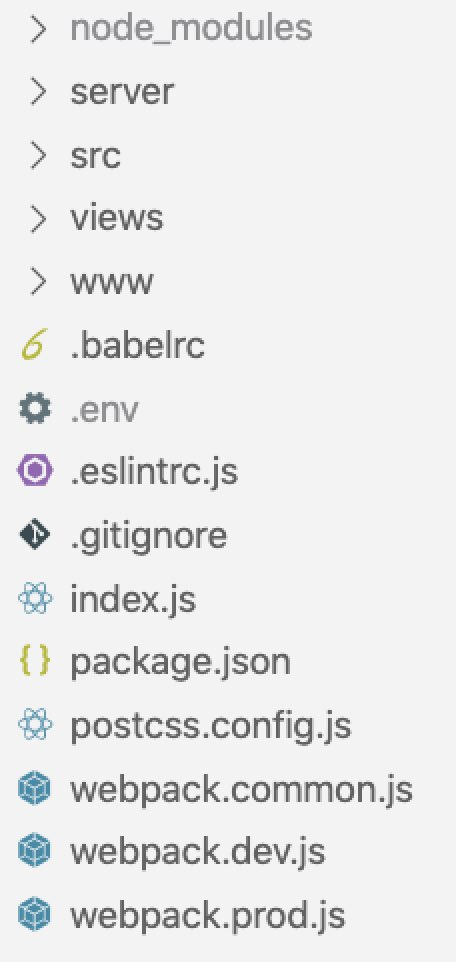
\includegraphics[width=0.3\textwidth]{app}
  \caption{Vista general de la raíz del proyecto.}
\end{figure}

\newpage
\subsubsection{Variables del entorno}
El acceso a las variables de entorno en Node.js es compatible desde el primer momento. Cuando el proceso Node.js se inicia, automáticamente proporciona acceso a todas las variables de entorno existentes al crear un objeto env como propiedad del objeto global del proceso.
\vspace{0.8cm}

\lstinputlisting[style=ES6, caption=Variables principales del sistema]{code/env.txt}


\newpage
\section{Configuración del servidor (Backend)}
Si alguna vez ha utilizado PHP o ASP, probablemente esté acostumbrado a la idea de que el servidor web (Apache o IIS, por ejemplo) sirve sus archivos estáticos para que un navegador puede verlos a través de la red. Node ofrece un paradigma diferente al de un servidor web tradicional: la aplicación es el servidor web. Node simplemente proporciona las bases para que se pueda construir un servidor web. 

\subsection{Servidor NodeJS}
El modelo de E/S impulsado por eventos sin bloqueo le brinda a NodeJS un rendimiento muy atractivo, superando fácilmente los entornos de servidores como PHP y Ruby on Rails, que bloquean las E/S y manejan múltiples usuarios simultáneos en hilos separados para cada uno. Algo importante que se debe saber es que NodeJS no es un \gls{framework} sino un entorno, hay \glspl{framework} que funcionan con Node, como Express y Sails, lo que facilita la creación de aplicaciones.
\vspace{0.8cm}

\begin{figure}[H]
  \centering
  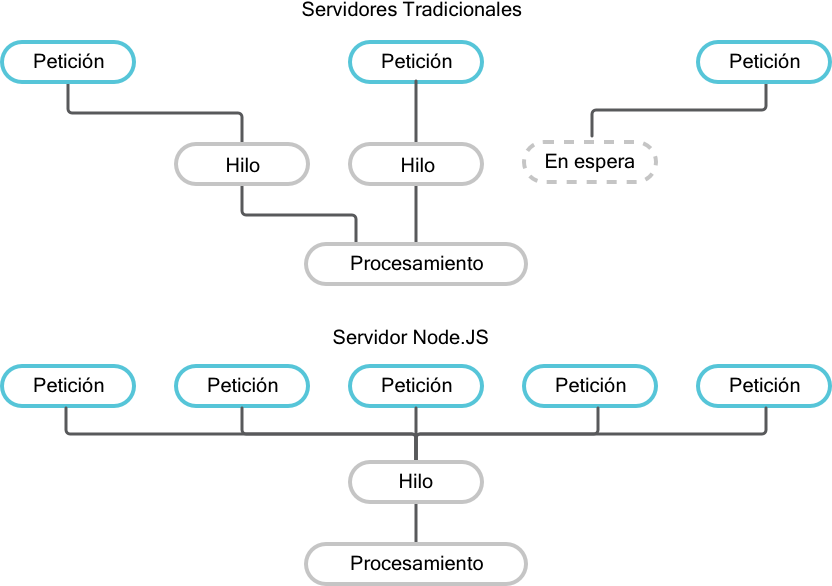
\includegraphics[width=0.8\textwidth]{node-traditional}
  \caption{Comparación de node y servidores tradicionales.}
\end{figure}

Un servidor Node.js tiene un solo subproceso de bucle de eventos (event-loop) que espera E/S en sockets y archivos. Una vez que los datos están listos, activa el método de evento correspondiente y espera hasta que regrese antes de esperar nuevamente por más eventos de E/S. Dado que todas las operaciones de E/S no bloquean, se asegurará de que todo se ejecute correctamente tan pronto como la entrada esté disponible sin ningún bloqueo y sin que se tenga lidiar con problemas de subprocesos múltiples.

\newpage
\subsubsection{Programación basada en eventos}
La filosofía central detrás de NodeJS es la programación basada en eventos. Significa que, el programador,  debe comprender qué eventos están disponibles y cómo responder a ellos. Muchas personas se introducen en la programación basada en eventos mediante la implementación de una interfaz de usuario: el usuario hace clic en algo y se dispara el `evento clic'. Es una buena metáfora, porque se entiende que el programador no tiene control sobre cuándo, o si el usuario va a hacer clic en algo, por lo que la programación basada en eventos es realmente bastante intuitiva \cite{ethan}.
\vspace{0.8cm}

\lstinputlisting[label={node-server}, style=ES6, caption=Configuración servidor NodeJS básico]{code/node-server.js}
En el ejemplo de código \ref{node-server}, el evento es implícito: el evento que se está manejando es una solicitud HTTP. El método http.createServer toma una función como argumento; esta función se invocará cada vez que se realice una solicitud HTTP. El programa simplemente establece el tipo de contenido en texto sin formato y envía la cadena `Hola, mundo!'.


\subsection{Configuración Express}
Express.js es un `marco de aplicación web NodeJS minimalista y flexible' \cite{express}. Es una capa delgada de características, fundamental para cualquier aplicación web, agrega tres características poderosas: enrutamiento, mejores manejadores de solicitudes y vistas.

\subsubsection{Enrutamiento}
Enrutamiento se refiere al mecanismo para servir al cliente el contenido que ha solicitado. Para las aplicaciones cliente/servidor basadas en web, el cliente especifica el contenido deseado en la URL (ruta y cadena de consulta).\\[0.8cm]
Cuando una aplicación Express.js se está ejecutando, escucha las solicitudes. Cada solicitud entrante se procesa de acuerdo con una cadena definida de middlewares y rutas que comienzan de arriba a abajo. Este aspecto es importante porque le permite controlar el flujo de ejecución \cite{azat}.
\vspace{0.8cm}

\begin{figure}[H]
  \centering
  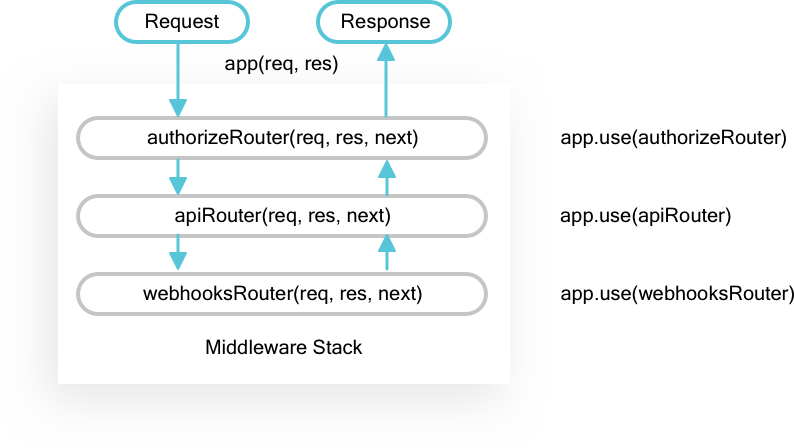
\includegraphics[width=0.8\textwidth]{express-router}
  \caption{Cada función de middleware en la pila se ejecuta antes que las que están debajo de ella. (Fuente: Elaboración propia)}
\end{figure}

\newpage
\lstinputlisting[style=ES6, caption=Fragmento de la configuración de enrutamiento del sistema]{code/express-router.js}

\subsection{Configuración Firebase}
Antes de conectar nuestro sistema con una base de datos de Firestore es necesario crear una aplicación en la consola de Google Firebase y seguir los siguientes pasos.
\vspace{0.8cm}

\begin{figure}[H]
  \centering
  
\includegraphics[width=1\textwidth]{firebase-01}
  \caption{Consola de Google Firebase.}
\end{figure}

\begin{enumerate}
  \item Crear un nuevo proyecto en la consola de Firebase.

  \begin{figure}[H]
    \centering
    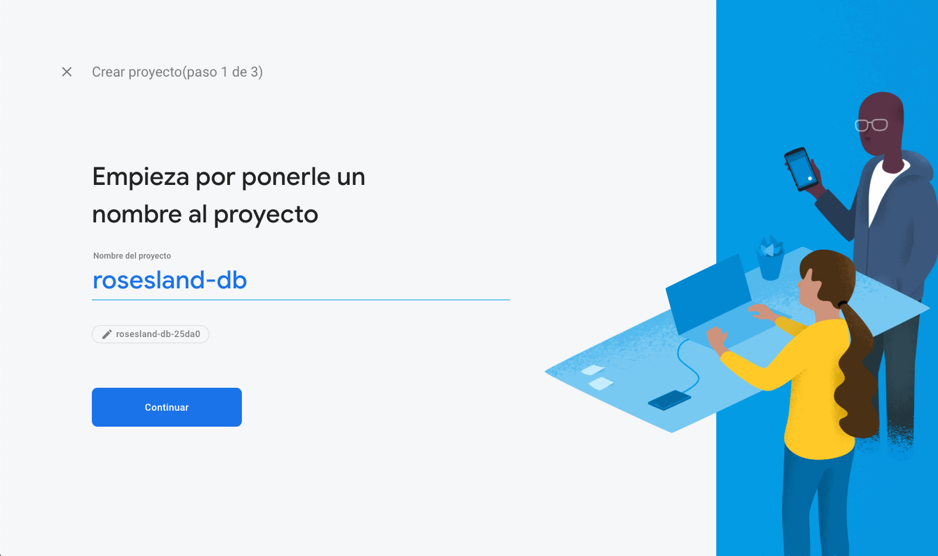
\includegraphics[width=1\textwidth]{firebase-02}
  \end{figure}

  \item En el apartado `Database', seleccionar `crear base de datos' .

  \begin{figure}[H]
    \centering
    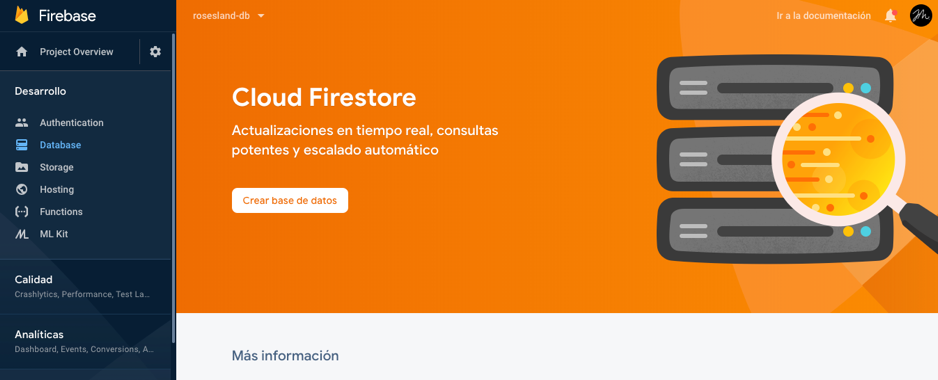
\includegraphics[width=1\textwidth]{firebase-03}
  \end{figure}

  \item En la ventana emergente, seleccionar reglas de seguridad y definir ubicación del servidor.

  \begin{figure}[H]
    \centering
    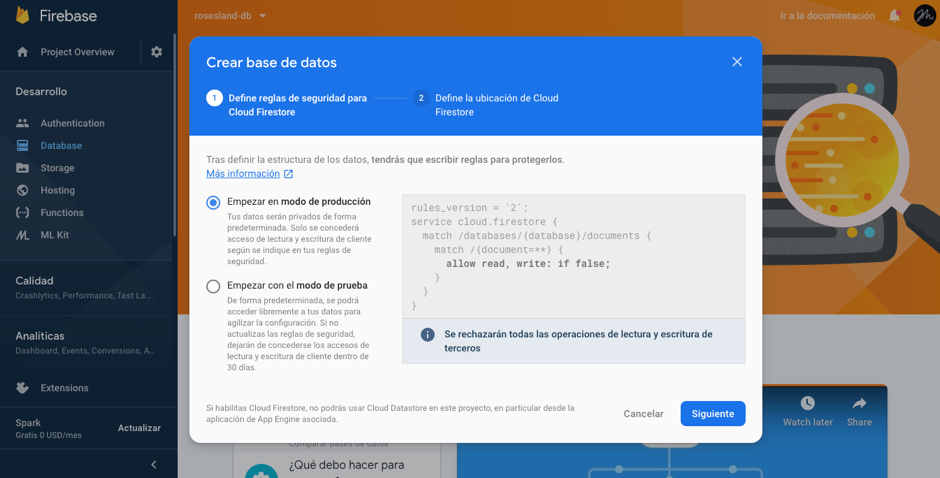
\includegraphics[width=1\textwidth]{firebase-04}
  \end{figure}

  \item El siguiente paso es generar las claves que permitan usar `firebase-admin' en el \textit{backend}. En la configuración del proyecto debajo del apartado `cuentas de servicio', presionar el botón `Generar cuentas de servicio'. El contenido del archivo JSON generado se debe de agregar a las variables del entorno que correspondan.

  \begin{figure}[H]
    \centering
    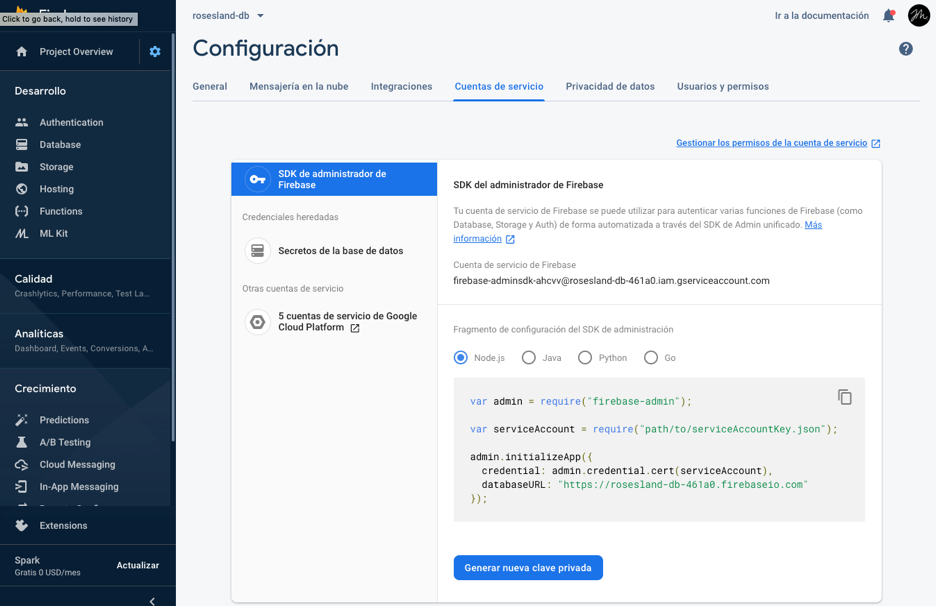
\includegraphics[width=1\textwidth]{firebase-05}
  \end{figure}

  \item Por ultimo en la sección `Authentication' se deben activar los servicios de autenticación necesarios, para este proyecto es necesario activar la validación por correo electrónico y contraseña.

  \begin{figure}[H]
    \centering
    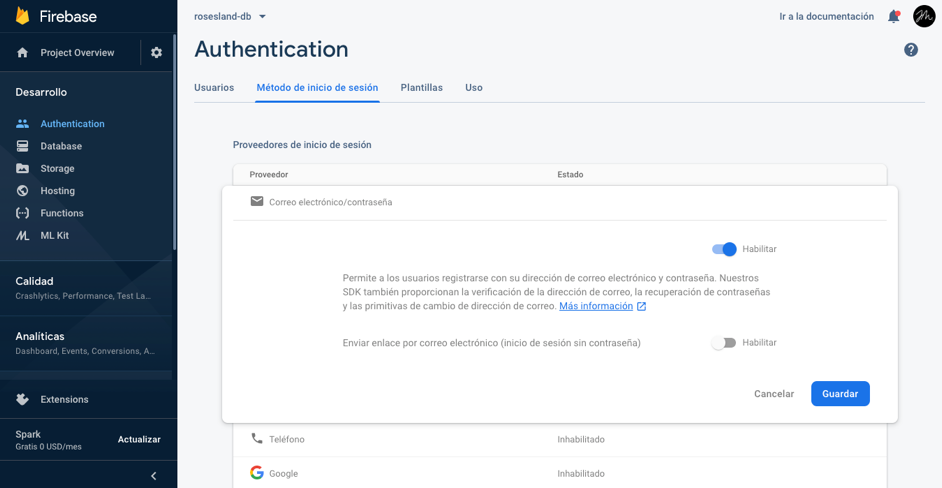
\includegraphics[width=1\textwidth]{firebase-06}
  \end{figure}
\end{enumerate}

\newpage
\subsubsection{Configuración de Firebase Firestore en Node.js}
Después de crear el objeto de configuración, es necesario inicializar Firebase en la aplicación de la siguiente manera:
\vspace{0.8cm}

\lstinputlisting[label={node-firebase}, style=ES6, caption=Fragmento de la configuración Firebase en el servidor]{code/firebase.js}

\subsubsection{Escrituras en lotes}
Para manipular documentos en un conjunto de operaciones, se pueden ejecutar varias operaciones de escritura como un lote único que incluya cualquier combinación de operaciones set(), update() o delete(). El lote de escrituras se completa de forma atómica y puede escribir en varios documentos. Los siguientes ejemplos muestran cómo crear y confirmar un lote de escrituras \cite{transactions}:
\vspace{0.8cm}

\lstinputlisting[label={firebase-function}, style=ES6, caption=Fragmento para guardar datos en Firestore]{code/firebase-function.js}


\subsection{Autenticación}
Casi todas las aplicaciones requieren algún sistema de autorización. En algunos casos, validar un nombre de usuario/contraseña establecido con nuestra tabla de Usuarios es suficiente, pero a menudo, necesitamos un modelo de permisos más detallado para permitir que ciertos usuarios accedan a ciertos recursos y los restrinjan de otros. Construir un sistema para soportar esto último no es trivial y puede llevar mucho tiempo. El API de autenticación basada en roles de Firebase, ayuda a poner todo en marcha rápidamente.

\subsubsection{Autenticación basada en roles}
En este modelo de autorización, se otorga acceso a roles, en lugar de usuarios específicos, y un usuario puede tener uno o más, según cómo diseñe su modelo de permiso. Los recursos, por otro lado, requieren ciertos roles para permitir que un usuario los ejecute.
\vspace{0.8cm}

\begin{figure}[H]
  \centering
  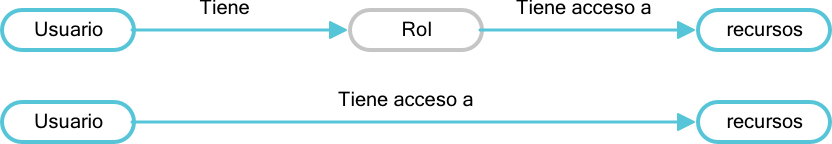
\includegraphics[width=1\textwidth]{firebase-auth}
  \caption{Autenticación basada en roles.}
\end{figure}

\subsubsection{Firebase Custom Claims}
Los roles de usuario son necesarios para identificar a los usuarios como administradores, gerentes o simplemente como clientes. Firebase Custom Claims permite establecer atributos de usuario simples directamente en el JWT del usuario (por ejemplo: \{ admin: true \}). Un JWT es un Json Web Token, es el objeto que contiene la información del usuario actual.
\vspace{0.8cm}

\lstinputlisting[label={firebase-auth}, style=ES6, caption=Fragmento para guardar crear y leer Firebase Custom Claims]{code/firebase-auth.js}

\subsection{Integración con Shopify}
La API de Storefront de Shopify brinda el control creativo completo para crear experiencias de compra personalizadas; se centra en las experiencias de compra vistas desde la perspectiva del cliente. Las características principales del API Storefront son \cite{storefront}:
\begin{itemize}
  \item Obtener datos sobre un solo producto o una colección de productos para mostrar en cualquier sitio web o dispositivo.
  \item Crear experiencias de pago únicas con control total sobre el carrito de compras.
  \item Crear nuevos clientes o modifique los existentes, incluida la información de la dirección.
\end{itemize}
Los motivos aquí son bastantes simples. Se requiere que los usuarios puedan navegar, buscar y seleccionar productos directamente en un dominio personalizado sin tener que ir a la tienda en linea de Shopify.
\vspace{0.8cm}

Una vez realizada una conexión exitosa con la API Storefront de Shopify, es posible crear componentes ReactJS para visualizar imágenes de productos, variaciones de productos, tamaños de productos, etcétera. De este modo el sistema podrá extender el uso de la plataforma.

\newpage
\lstinputlisting[label={node-shopify}, style=ES6, caption=Fragmento de código para la conexión con Shopify]{code/shopify.js}

\subsection{Webhooks}
Un webhook permite que servicios de terceros envíen actualizaciones en tiempo real a su aplicación. Las actualizaciones se activan por algún evento o acción por parte del proveedor de webhook, y se envían a su aplicación a través de solicitudes HTTP. Cuando recibe la solicitud, la maneja con una lógica personalizada, como enviar un correo electrónico o almacenar los datos en una base de datos.

\subsection{Webhooks Shopify}
Un webhook se puede usar para recibir notificaciones sobre eventos particulares en una tienda en linea. Después de suscribirse a un webhook, puede permitir que su aplicación ejecute código inmediatamente después de que ocurran eventos específicos en las tiendas que tienen su aplicación instalada, en lugar de tener que hacer llamadas \acrshort{api} periódicamente para verificar su estado. Por ejemplo, puede configurar un webhook para activar una acción en su aplicación cuando un cliente crea un carrito de compras o cuando un comerciante cree un nuevo producto en su administrador de Shopify. Al usar las suscripciones de webhooks, puede hacer menos llamadas \acrshort{api} en general, lo que garantiza que la aplicación sea más eficiente y se actualice rápidamente \cite{webhook}.
\vspace{0.8cm}

\begin{figure}[H]
  \centering
  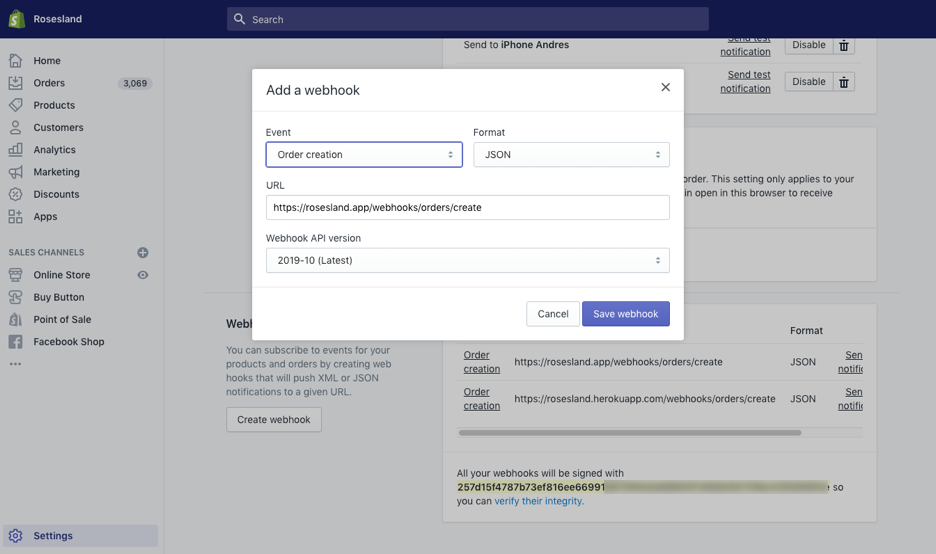
\includegraphics[width=1\textwidth]{webhook}
  \caption{Panel para crear webhooks en Shopify. (Fuente: Shopify Admin)}
\end{figure}

Después de configurar una suscripción de webhook, los eventos que especificó activarán una notificación de webhook cada vez que ocurran. Esta notificación contiene información JSON y encabezados HTTP que proporcionan contexto.

\newpage
\subsection{Configuración de webhook en Express.js}
En lugar de extraer información a través del \acrshort{api}, los webhooks enviarán información a su punto final.
\vspace{0.8cm}

\lstinputlisting[style=ES6, caption=Ruta que capta el webhook lanzado desde Shopify]{code/webhook.js}

\subsection{Websockets con Socket.IO}
Si bien la base de datos Firebase Firestore proporciona una capa de conexión en tiempo real, es necesario introducir un nuevo método de comunicación permanente para notificar de eventos como lo son la presencia de usuarios activos y la visualización de las ordenes. Socket.IO permite la comunicación bidireccional entre el cliente y el servidor. Las comunicaciones bidireccionales se habilitan cuando un cliente tiene Socket.IO en el navegador, y un servidor también ha integrado el paquete. Si bien los datos se pueden enviar de varias formas, JSON es el más simple. Resume muchos tipos de transportes, incluidos AJAX y WebSockets, en una sola API. Permite a los desarrolladores enviar y recibir datos sin preocuparse por la compatibilidad entre navegadores \cite{kelleher}.
\vspace{0.8cm}

En cualquier aplicación en tiempo real, mostrar múltiples usuarios en línea es muy importante, esta información debe actualizarse cuando un nuevo usuario se conecta o un usuario en línea se desconecta.
\vspace{0.8cm}

\lstinputlisting[style=ES6, caption=Fragmento de configuración de Socket.IO del sistema]{code/socket.js}

\newpage
\section{Patrones de diseño}
Los patrones de diseño facilitan la reutilización de diseños y arquitecturas exitosas. Los patrones de diseño ayudan a elegir alternativas de diseño que hacen que un sistema sea reutilizable y evitar alternativas que comprometan la reutilización. Pueden incluso mejorar la documentación y el mantenimiento de los sistemas existentes.
\subsection{Redux}
Redux es un administrador de estado predecible para aplicaciones JavaScript basado en el patrón de diseño Flux. A medida que una aplicación crece, se hace difícil mantenerla organizada y mantener el flujo de datos. Redux resuelve este problema administrando el estado de la aplicación con un único objeto global llamado Store. Los principios fundamentales de Redux ayudan a mantener la coherencia en toda la aplicación, lo que facilita la depuración y las pruebas.
\subsubsection{Redux Store}
Redux Store contiene un objeto del estado global de la aplicación. Esta actualiza el estado y notifica los componentes suscritos. \\[0.8cm]
\lstinputlisting[style=ES6, caption=Fragmento de código para inicializar el Store]{code/redux-store.js}

\subsubsection{Redux Reducer}
Un Reducer es solo una función pura de JavaScript. Recibe dos parámetros: el estado actual y la acción. Una función pura es aquella que devuelve exactamente la misma salida para la entrada dada. El estado es el objeto Store completo, la acción es el objeto despachado con un tipo requerido y un payload opcional. \\[0.8cm]
\lstinputlisting[style=ES6, caption=Fragmento de código del reducer común de la app]{code/redux-reducer.js}

\subsubsection{Acciones Redux}
La única forma de cambiar el estado es enviando una señal a el Store. Esta señal es una acción. Entonces "despachar una acción" significa enviar una señal a el Store. \\[0.8cm]
\lstinputlisting[style=ES6, caption=Fragmento de código de la acción que valida a un administrador]{code/redux-action.js}


\newpage
\section{Integración React/Redux}
Para conectar el Store de Redux con React, es mediante un componente llamado Provider. El único propósito de Provider es agregar el Store al contexto del componente de la Aplicación, para que todos los componentes secundarios puedan acceder a ella. Provider envuelve a la aplicación React y hace que sea consciente de el Store. \\[0.8cm]
\lstinputlisting[style=ES6, caption=Fragmento de código de la aplicación React principal]{code/redux-react.js}



\chapter{Conclusiones}
El objetivo del proyecto era desarrollar y desplegar un sistema en la empresa Rosesland que les permitiera llevar un proceso de trabajo más automatizado. Esta compañía de venta de arreglos florales, como muchas organizaciones, necesitaba migrar sistemas operativos clave a plataformas web para aprovechar beneficios como la ubicuidad del acceso web y la arquitectura orientada a servicios. Para lograr esto, se desarrolló un servidor basado en Node.js que se conecta con los servicios de venta en linea de Shopify, así como una aplicación web creada con React.js siguiendo la metodología del diseño atómico e implementando Redux para el manejo del estado, el sistema utiliza los servicios de Google Firebase para la autenticación y el almacenamiento de los datos.
\vspace{0.8cm}

Los servicios de venta en linea son cada vez mas populares tanto en tiendas minoristas como en mayoristas,  este sistema se enfocó en mejorar la situación laboral de los empleados y ofrecer un servicio mas agradable a los clientes. Se canalizaron principios de usabilidad en una web de ventas para crear una plataforma que influye positivamente en el uso de el sistema como herramienta para los trabajadores. Una vez finalizadas las pruebas y haber garantizado el funcionamiento de todos los módulos se puede concluir que se obtuvieron los resultados deseados. El sistema tuvo un gran desempeño y todas las actividades de la empresa fueron mas fáciles de realizar. Uno de los principales beneficios que aporta se ve reflejado en la capacidad para analizar y administrar las ventas como antes no se había imaginado.
\vspace{0.8cm}

Conforme el proyecto evolucionaba en su proceso de desarrollo, pruebas y ejecución, se adquirieron conocimientos importantes. Los procedimientos establecidos al crear este proyecto sirven como base para elaborar otras aplicaciones, su código es escalable y permite integrar un gran numero de servicios y frameworks, por lo que su limitación solo estará marcada por las necesidades de los usuarios.
\vspace{0.8cm}



\printbibliography

\printglossary

\clearpage

\printglossary[type=\acronymtype]

\end{document}